\documentclass[12pt]{article}

\usepackage{polyglossia}
\setmainlanguage{english}

\usepackage{parskip}
\setlength{\parskip}{2ex}
\setlength{\parindent}{0em}

\usepackage{graphicx}
\graphicspath{ {./images/} }

\widowpenalty=10000
\clubpenalty=10000

\input{title-page-settings.inc}

\begin{document}

\maketitle

\clearpage

\section*{Purpose}

We were assigned this project to make the overall student experience with planning their college career better. Right now, students in the computer science department are given a flowchart for a general structure of what each semester should look like. Our goal is to turn this into a website that adds customization and clarity that also follows the rules of what you can take.

A common problem with the current system is, incoming and current students get confused with what the courses can be taken that also go within the restrictive electives. With this online flow chart, you will be able to select the elective list name and have all the available classes for that slot show up, move classes around freely that don’t violate any of the rules and be able to generate a test schedule for their next semester.


\section{Flowchart}

The main functionality of this project revolves around the flowchart. This will allow for students to plan out their college career as many years in advance as they’d like. 

\begin{enumerate}
    \item This involves the student choosing a plan that they would like to follow. Currently, we only have CIS as a valid career path, so this is the only available choice.
    \item After the plan is chosen, the flowchart is then populated with a modeled version of these requirements known as Plan Requirements. These are then displayed on the flowchart screen as the boxes with the different information on it.
    \begin{enumerate}
        \item Currently this is where the bulk of the functionality exists. These classes are then connected in many different ways to different models to give us different functionality. You will notice on the Flowchart that there are different buttons for each class. Some classes have different prerequisites, among other properties.
        \item You will also notice that there are different semesters that can be changed as well. This also factors into the different rule checks that happen. If a semester is created and it is empty, a new button will appear on the semester box that will allow the creation of a summer semester
        \begin{enumerate}
            \item These summer semesters act differently than normal semesters. You may notice that as semesters are dragged around and reordered, the semester and year of the semester changes dynamically as well. Normally, the semesters will change to the proper order if they are ‘Fall’ or ‘Spring’ along with the year, but summer semesters always stay as summer semesters and only the year changes for them.
        \end{enumerate}
    \end{enumerate}
    \item All of these properties are then used to run through different rule checks to make sure that the plan is valid. These include things like not taking a class that has a prerequisite that the student doesn't have, making sure that enough hours are being taken per semester, checking to make sure that all K-State and College of Engineering requirements are met. This allows the validation of the student’s flowchart so they know if their plan is valid or not.
    \item You may notice that there are different types of classes on the flowchart. Some already have a class chosen, while others just appear to be a generic gen ed class. The classes that are already chosen are those that are required for the plan requirements and the electives are the same, but because the student has not chosen a class to take for those electives they just appear as a generic elective class. The rules should be able to know that these classes should be counted as the proper electives required as long as their Course value hasn't been set.
    \begin{enumerate}
        \item All of the Plan Requirements objects can have connection to Course objects, and you may notice when you edit a class on the flowchart you are presented with a dialog box. On that dialog box among other fields you will see the Course Match and Completed Course Match
        \begin{enumerate}
            \item Each one of these objects on the flowchart can map to both. The classes that are filled from the beginning have the course match set already but do not have Completed Course Match.
            \begin{enumerate}
                \item The completed course matches are set later through the dashboard. These completed classes are also run through the rules, especially at the end to check to make sure that all of the Plan Requirements and the K-State requirements are fulfilled before graduation
            \end{enumerate}
            \item We are currently working on a feature for the Course Match and Course Completed match that will change the implementation of the auto-fill to only suggest classes that either: match the elective list, or match the class itself (if the class is required i.e. CIS 200, then we only want that class to be the Completed Course or Course match
        \end{enumerate}
    \end{enumerate}
\end{enumerate}

\begin{figure}
    \centering
    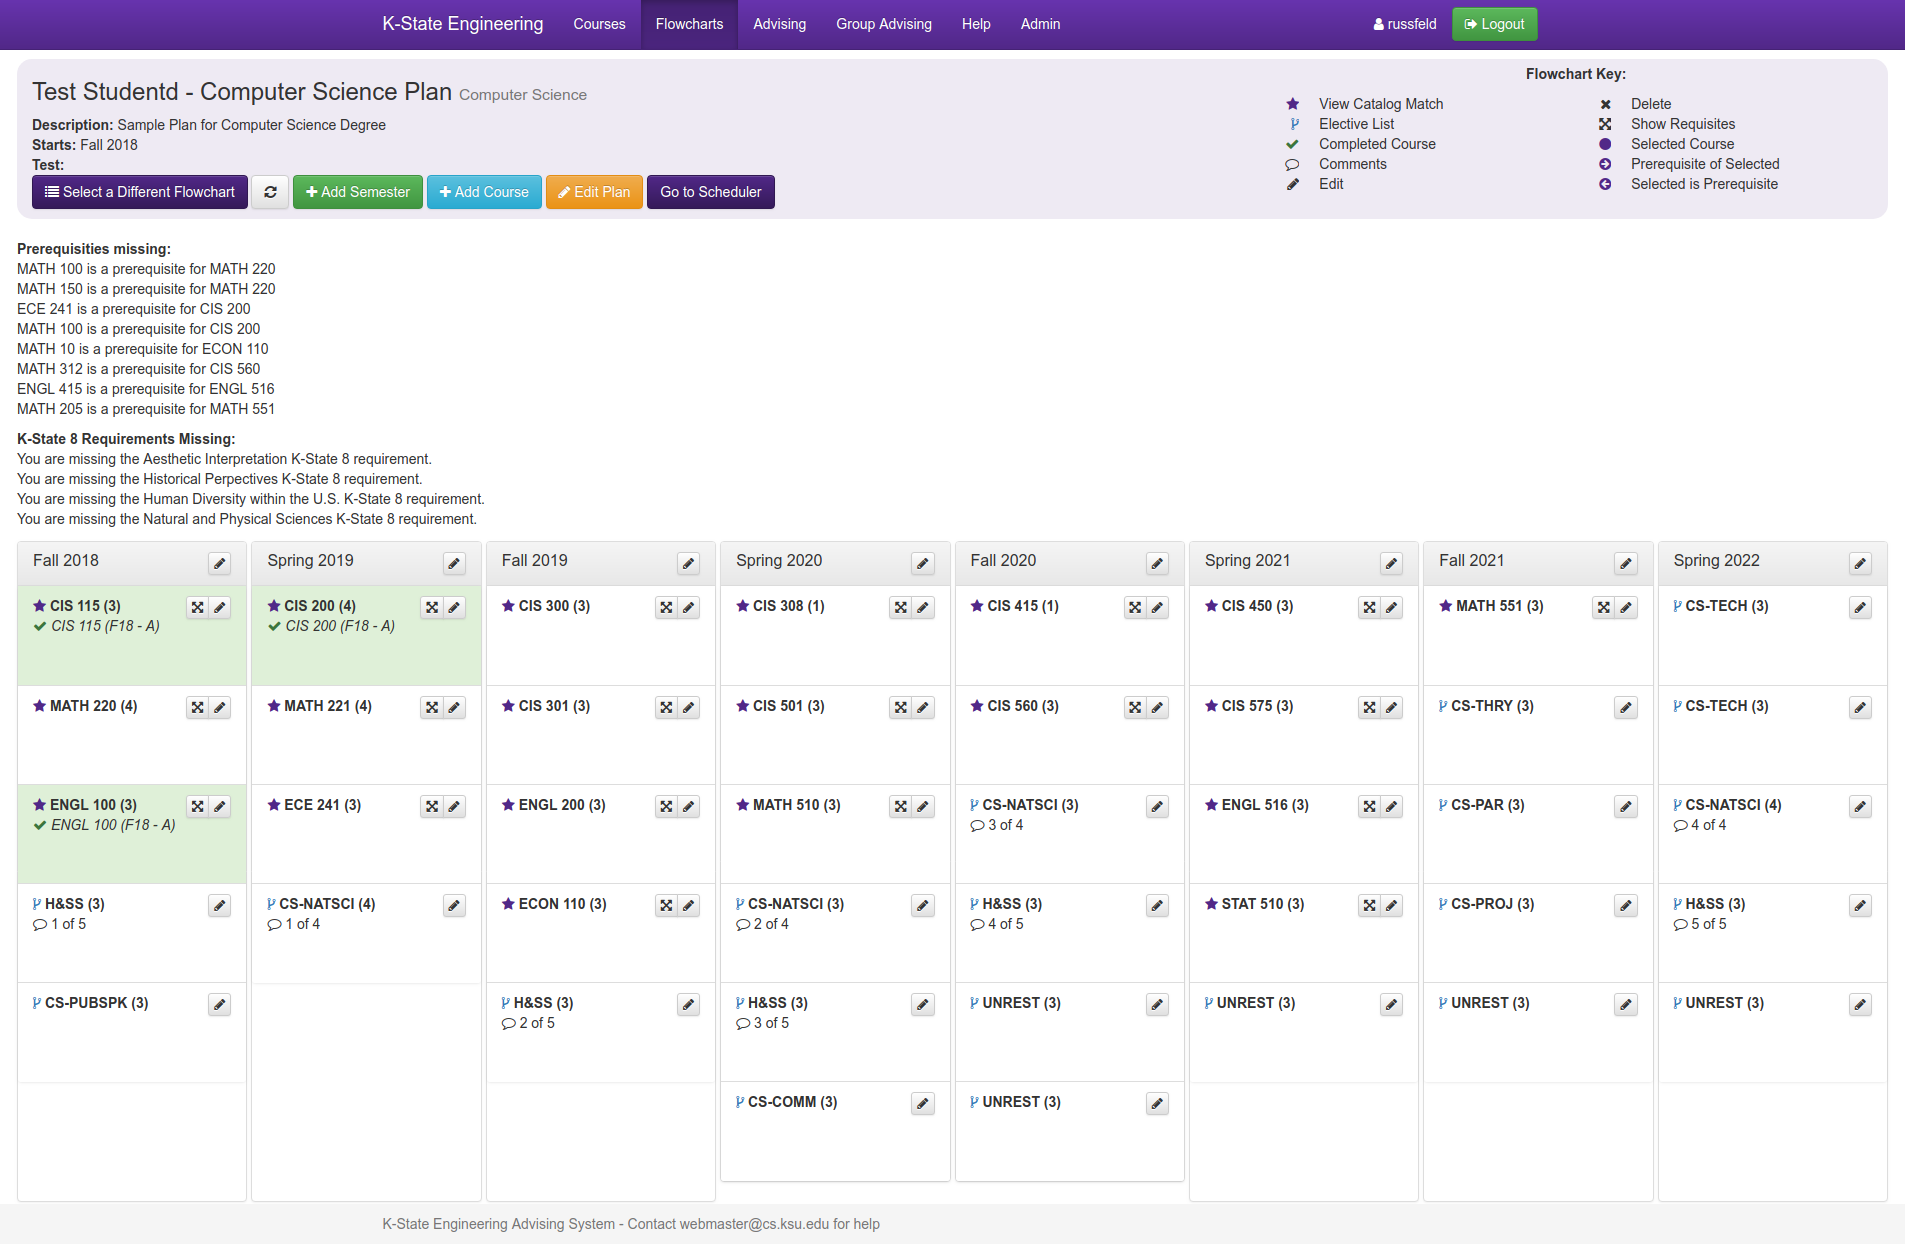
\includegraphics[width=\textwidth]{flowchart.png}
    \caption{Flowchart view}
    \label{fig:flowchart}
\end{figure}


\section{Scheduler}

The purpose of the scheduler is to give the students a view to look at to make their schedule for a semester. To do this, we made a weekly calendar view for the class to be displayed on. With this calendar, you will be able to search for any class at Kansas State. The results will be displayed below the search with the information about the class and times it is offered. With this, you will be able to click on a class and it will be added to your schedule.

The way we get all the classes and their times are from a scraper. We scrape the course catalog then store all the info into our database. The scraper will run before every semester when the catalog is updated. This will make sure class information will stay up to date.

For future functionality, we want it to be able to take the classes from the students flowchart for the next semester and add them to the calendar. This will automatically generate a test schedule for the student, if they don’t like it, they will be able to change by deleting a class and searching for a new one with the search function.

\begin{figure}
    \centering
    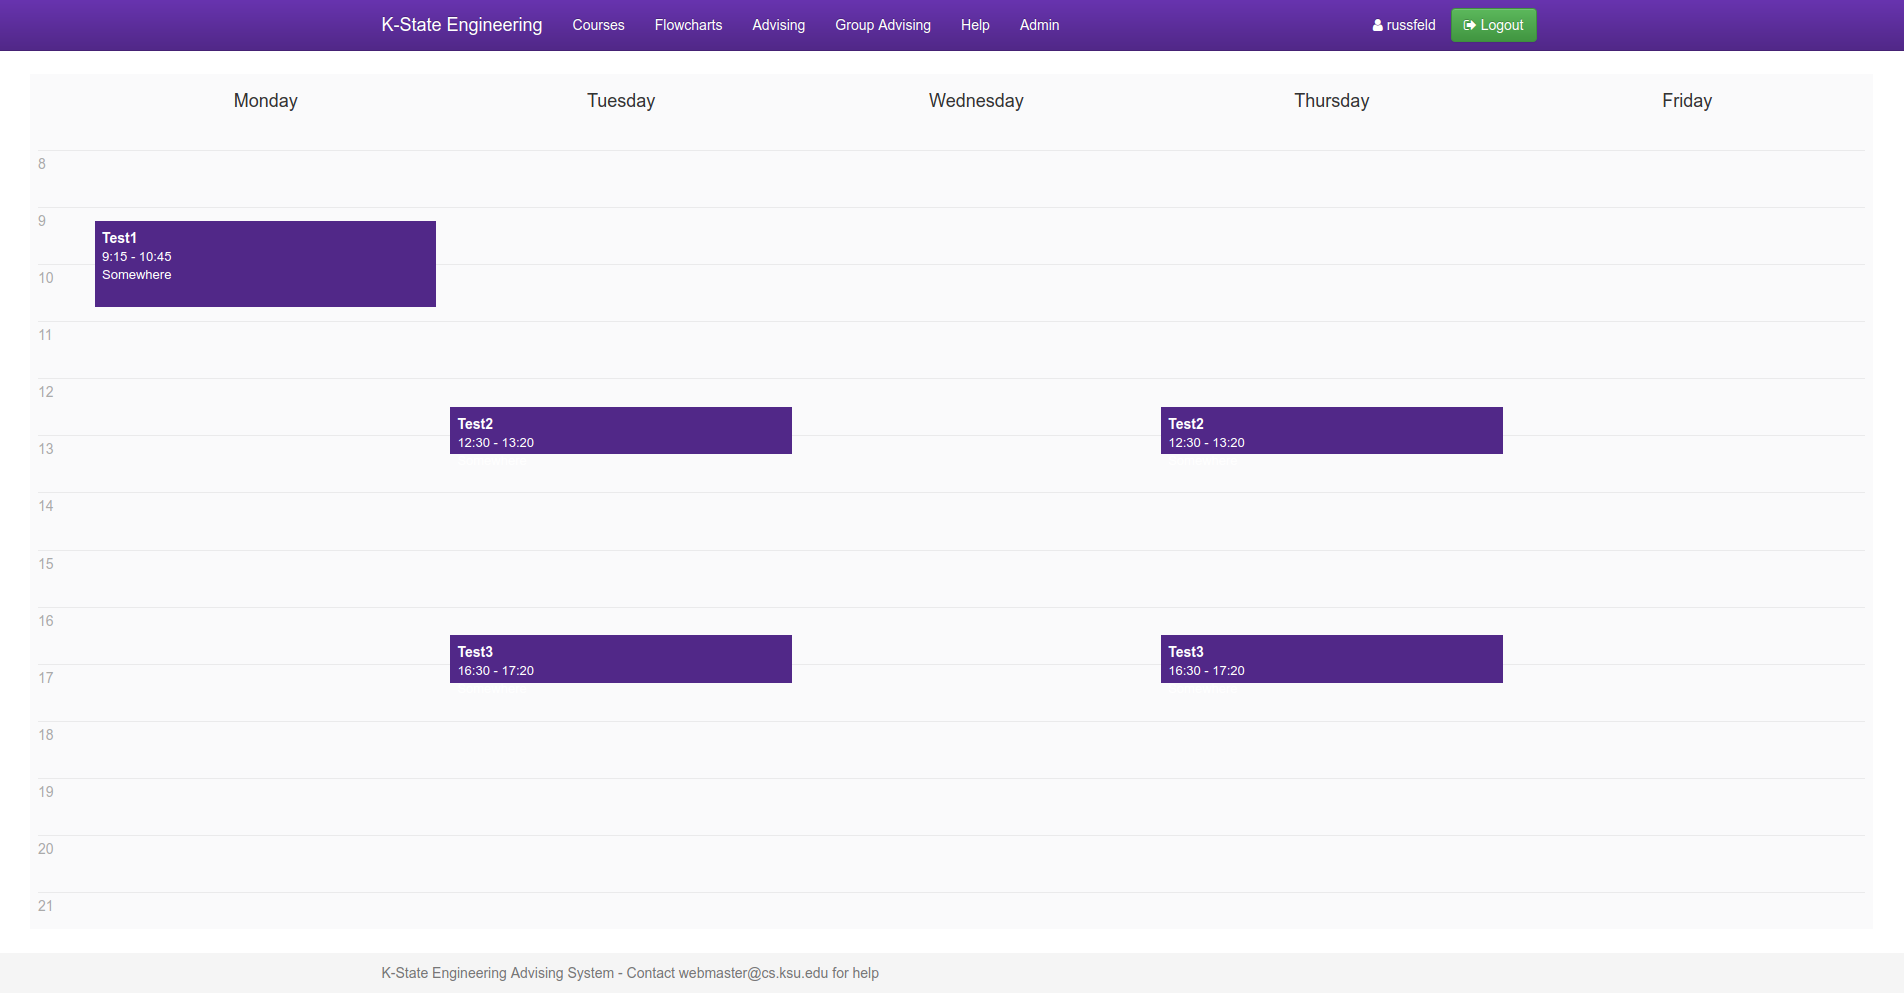
\includegraphics[width=\textwidth]{semester.png}
    \caption{Semester classes scheduler view}
    \label{fig:semester}
\end{figure}

\section{Advising}

In the advising section, advisors can review their schedule and see the the scheduled meetings and blackouts. They can also schedule new meeting and blackout.

Students can see their assigned advisor. However, they can see all the available advisors and schedule a meeting with anyone of them.

\begin{figure}
    \centering
    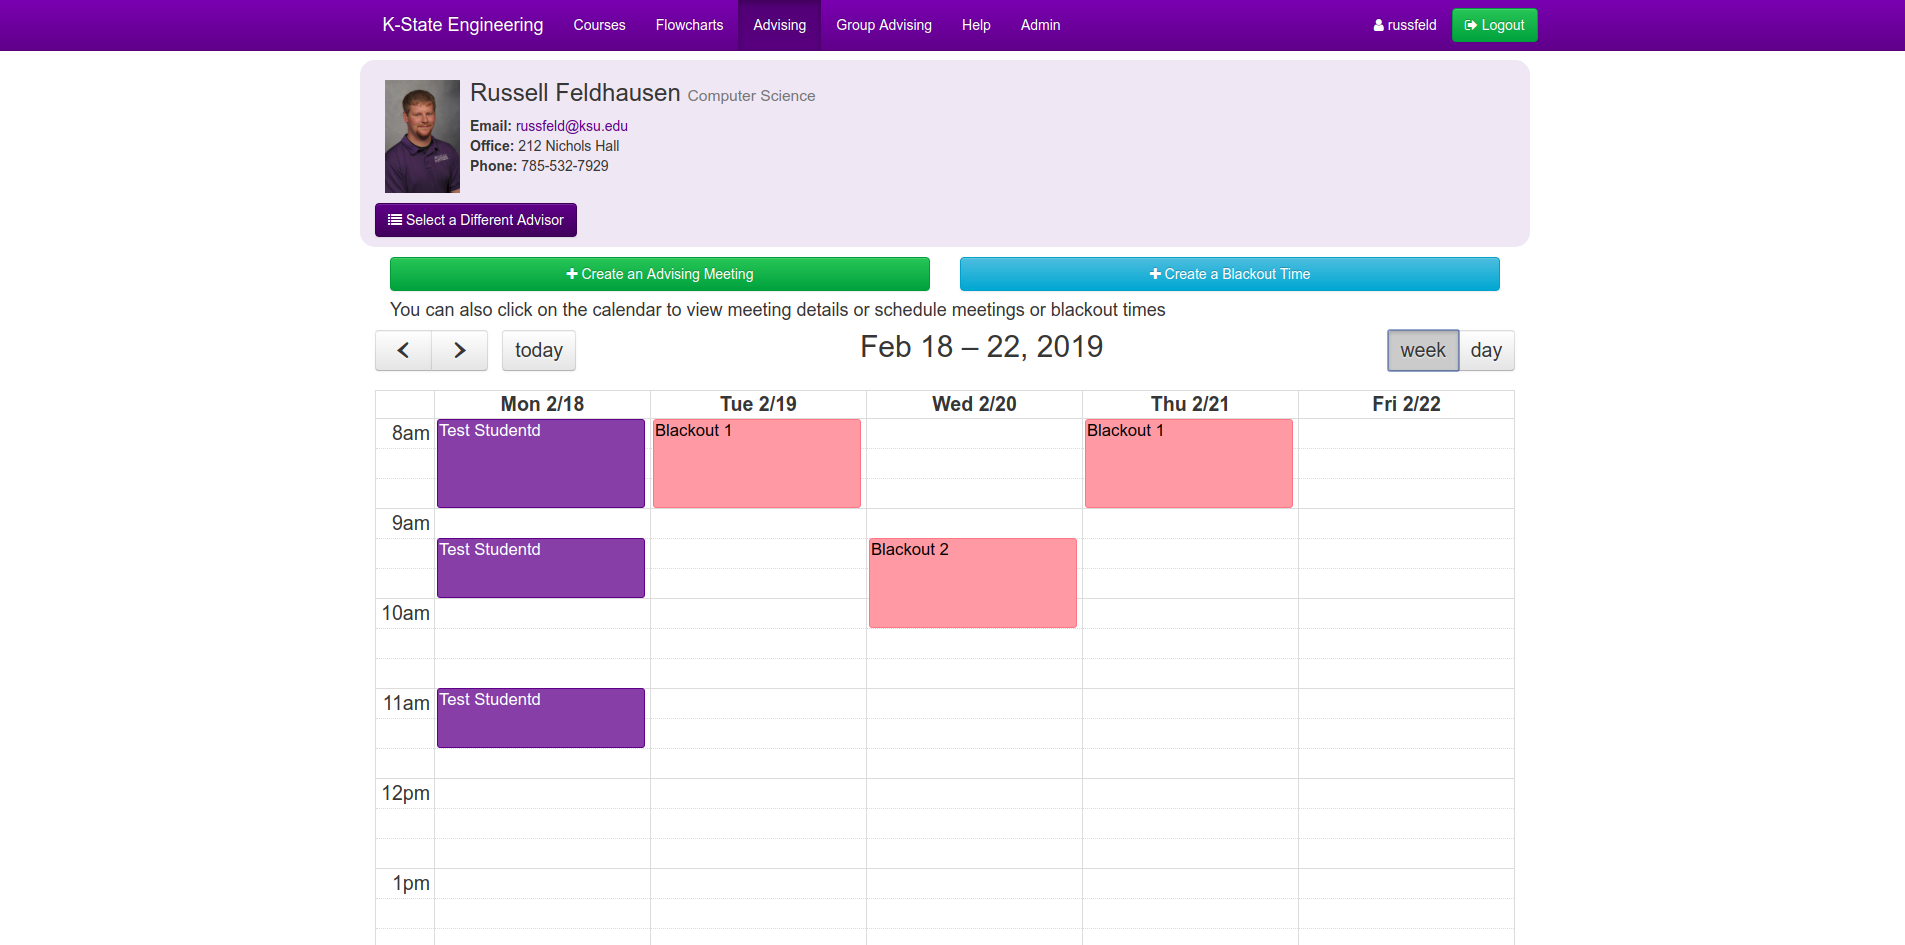
\includegraphics[width=\textwidth]{advising-advisor.png}
    \caption{Advising section as seen by advisors}
    \label{fig:advisor}
\end{figure}

\begin{figure}
    \centering
    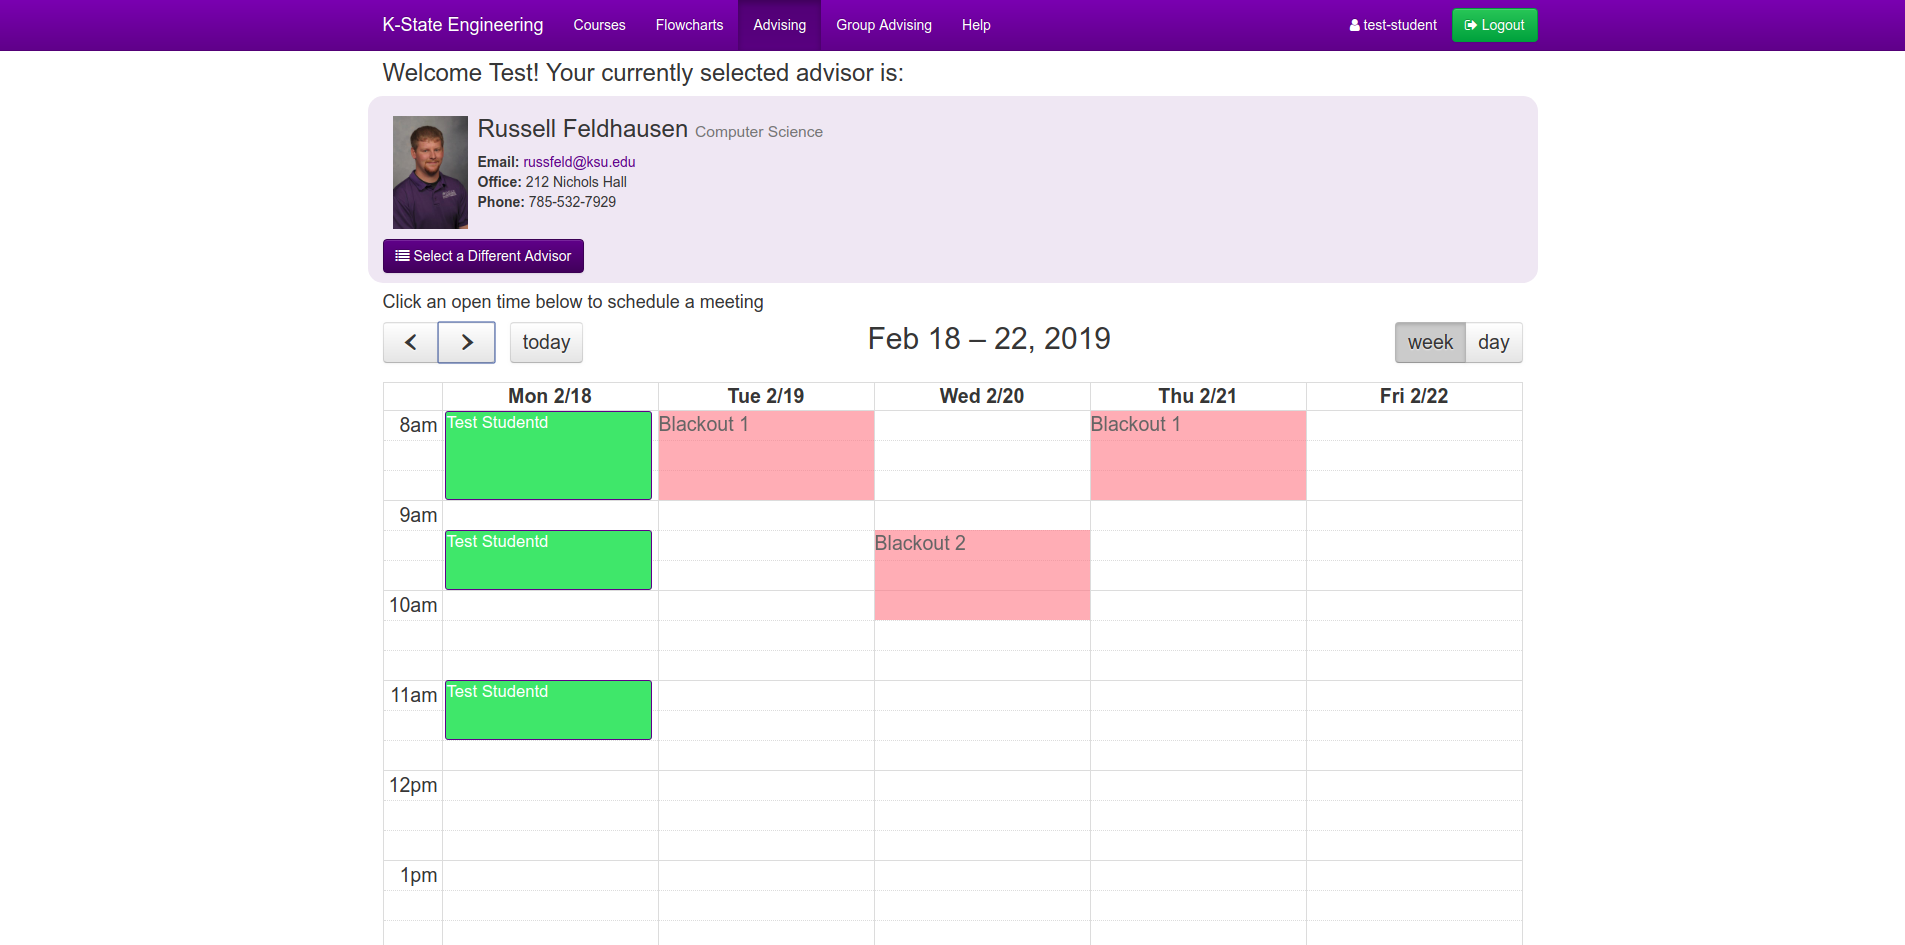
\includegraphics[width=\textwidth]{advising-student.png}
    \caption{Advising section as seen by students}
    \label{fig:student}
\end{figure}


\section{Administration}
Administration section serves the administrators of the portal and allows them to manage users, both advisors and students, i.e., create new user, modify or delete exiting one. Each user is assigned to a department; the departments can be created, modified and deleted as well. Next, the administrator can see, modify, create and delete students' plans, degree programs, elective lists.

The administrators can also review and delete any and all of the scheduled advising meetings, group sessions and blackouts.

\begin{figure}
    \centering
    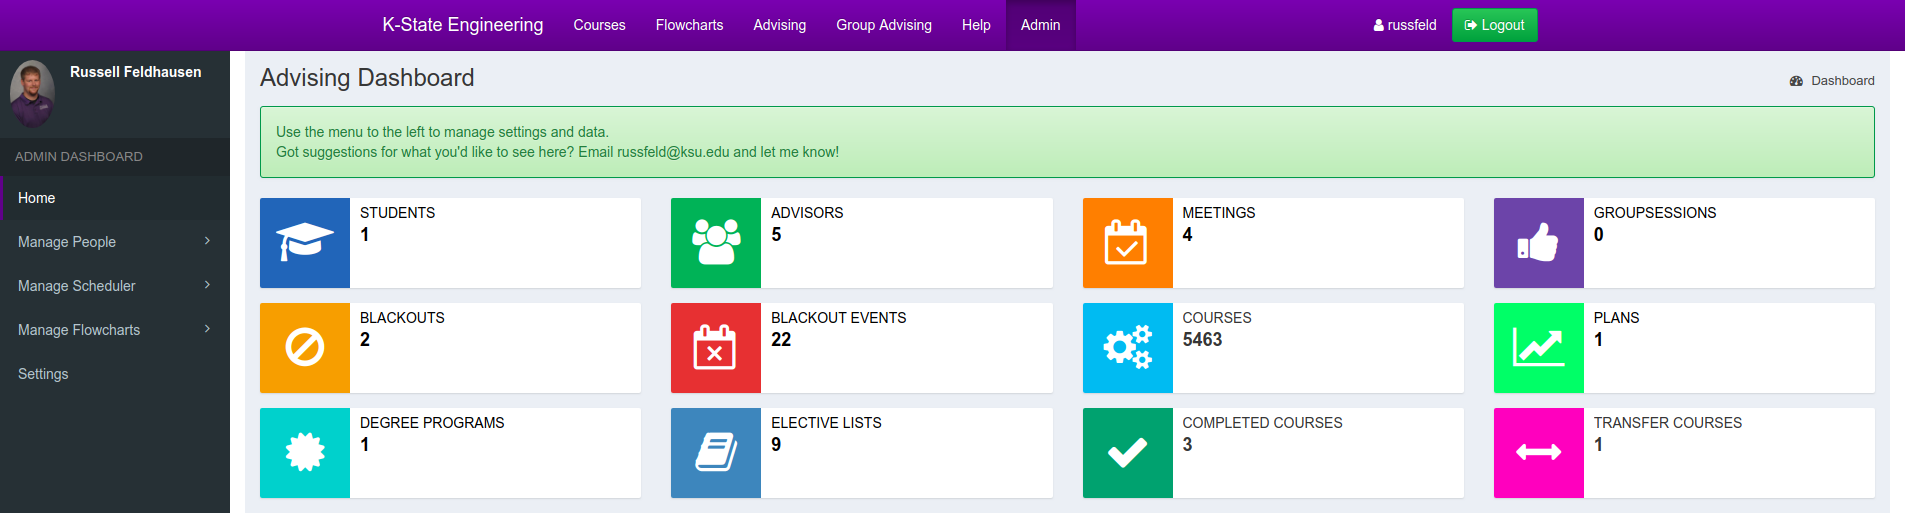
\includegraphics[width=\textwidth]{administration.png}
    \caption{Administration}
    \label{fig:administration}
\end{figure}

\end{document}
